\section{System Architecture}

\begin{figure*}[h!]
    \begin{center}
        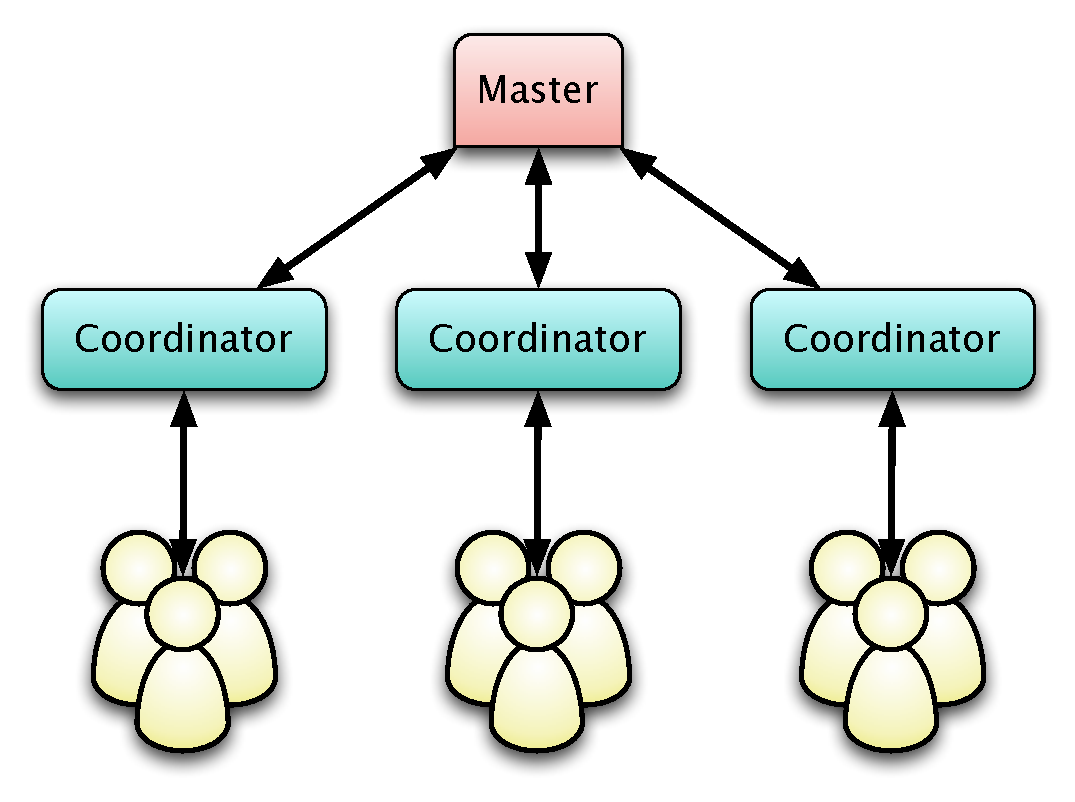
\includegraphics[width=3in]{figures/arch0.pdf}
    \end{center}
    \caption{Basic architecture of the system.}
    \label{arch}
\end{figure*}

Part of this project will include dynamically balancing the load of communication between agents and
coordinators. There are at least three possible approaches to this problem in the context of this
simulation.

The simplest way to assign agents to coordinators is to assign a constant number of agents to each
agent coordinator at random or based on some positioning heuristic. No agents will ever change their
coordinators. This strategy would create significant overhead from passing messages between agents
on separate coordinators.

\begin{figure*}[h!]
    \begin{center}
        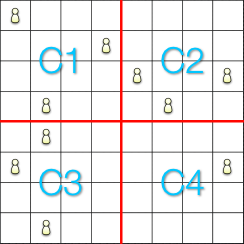
\includegraphics[width=3in]{figures/arch1.png}
    \end{center}
    \caption{Grid-based method for distributing work across coordinators}
    \label{geoarch}
\end{figure*}

A more efficient strategy would be to assign each coordinator a section of the grid and have
coordinators hand off responsibility for agents at the borders between coordinators. This way,
coordinators would only need to exchange agent messages when the agents are near coordinator
borders. One downside of this strategy is that some coordinators may be responsible for many more
agents than others if agents cluster in a few areas.

This problem could be solved by allowing the master process to dynamically reallocate the space
assigned to each coordinator. \textbf{This dynamic reassignment is very similar to the problem of
assigning many application instances to many servers,} but in addition to simply trying to
distribute CPU and memory load evenly, we are also trying to reduce the traffic between servers
which must pass data to each other (agent broadcasts) for the simulation to be correct.
